\documentclass[11pt,a4paper]{article}
\usepackage[top=3cm, bottom=2cm, left=2cm, right=2cm]{geometry}
\usepackage[utf8]{inputenc}
\usepackage{amsmath, amsfonts, amssymb}
\usepackage{siunitx}
\usepackage[brazil]{babel}
\usepackage{graphicx}
\usepackage[margin=10pt,font={small, it},labelfont=bf, textfont=it]{caption}
\usepackage[dvipsnames, svgnames]{xcolor}
\DeclareCaptionFont{MediumOrchid}{\color[svgnames]{MediumOrchid}}
\usepackage[pdftex]{hyperref}
\usepackage{natbib}
\bibliographystyle{plainnat}
\bibpunct{\textcolor{MediumOrchid}{\textbf{[}}}{\textcolor{MediumOrchid}{\textbf{]}}}{,}{s}{}{}
\usepackage{color}
\usepackage{footnote}
\usepackage{setspace}
\usepackage{booktabs}
\usepackage{multirow}
\usepackage{subfigure}
\usepackage{fancyhdr}
\usepackage{leading}
\usepackage{indentfirst}
\usepackage{wrapfig}
\usepackage{mdframed}
\usepackage{etoolbox}
\usepackage[version=4]{mhchem}
\usepackage{enumitem}
\usepackage{caption}
\usepackage{titlesec}
\usepackage{tcolorbox}
\usepackage{tikz}
\usepackage{LobsterTwo}
\usepackage[T1]{fontenc}
\usepackage{fontspec}
\usepackage{txfonts}
\usepackage[bottom]{footmisc}

\makeatletter
\def\footnoterule{\kern-3pt\color{MediumOrchid}\hrule\@width0.6\textwidth height 0.8pt\kern2.6pt}
\makeatother

\renewcommand{\footnotelayout}{\itshape\color{black}}

\AtBeginEnvironment{equation}{\fontsize{13}{16}\selectfont}


\titleformat{\section}{\LobsterTwo\LARGE\color{CarnationPink}}{\thesection.}{1em}{}
\titleformat{\subsection}{\LobsterTwo\LARGE\color{CarnationPink}}{\thesubsection}{1em}{}


\DeclareCaptionLabelFormat{figuras}{\textcolor{DarkTurquoise}{Figura \arabic{figure}}}
\captionsetup[figure]{labelformat=figuras}

\makeatletter
\renewcommand\tagform@[1]{\maketag@@@{\color{CarnationPink}(#1)}}
\makeatother

\renewcommand{\theequation}{Eq. \arabic{equation}}
\renewcommand{\thefigure}{Fig. \arabic{figure}}
\renewcommand{\thesection}{\textcolor{CarnationPink}{\arabic{section}}}

\setlist[itemize]{label=\textcolor{CarnationPink}{$\blacksquare$}}

\setlist[enumerate]{label=\textcolor{CarnationPink}{\arabic*.}, align=left, leftmargin=1.5cm}


\newcounter{exemplo}

\NewDocumentEnvironment{exemplo}{ O{} }{%
\allowbreak
\setlength{\parindent}{0pt}
  \begin{mdframed}[
  leftline=true,
  topline=false,
  rightline=false,
  bottomline=false,
  linewidth=2pt,
  linecolor=CarnationPink,
  frametitlerule=false,
  frametitlefont=\LobsterTwo\large\color{CarnationPink},
  frametitle={\color{CarnationPink}\LobsterTwo\large #1},
  ]
}{%
  \end{mdframed}
}

\setlength{\fboxsep}{5pt}
\setlength{\fboxrule}{1.5pt}
\usepackage{float}
\renewcommand{\thefootnote}{\alph{footnote}}
\usepackage{url}
\hypersetup{
	colorlinks=true,
	linkcolor=DarkTurquoise,
	filecolor=DarkTurquoise,      
	urlcolor=DarkTurquoise,
	citecolor=DarkTurquoise,
	pdftitle={Especialista em Física da Radioterapia}
}
\pagestyle{fancy}
\fancyhf{}
\renewcommand{\headrulewidth}{0pt}
\rfoot{Página \thepage}

\title{\LobsterTwo\Huge{Radiobiologia}}
\author{\LobsterTwo\Large{Curvas de Sobrevivência Celular}\nocite{*}}
\date{\LobsterTwo\textit{Dalila Mendonça}}
\begin{document}
	\maketitle

\section{Modelos Baseados Na Distribuição de Poisson}

	Os modelos matemáticos de sobrevivência celular após irradiação mais abordados são: single-hit multitarget, dois componentes, linear-quadrático e modelos de dose biologicamente efetiva ou equivalente. Todos esses modelos matemáticos são maneiras diferentes de interpretar os dados disponíveis (sobrevivência celular, controle do tumor, \dots).

  	O modelo mais comum e mais simples utilizado na rotina clínica é o \textcolor{DarkTurquoise}{\Large\LobsterTwo\textbf{modelo linear-quadrático ($\mathbf\mathrm{\alpha/beta}$)}}, porém existem modelos mais sofisticados na literatura. 

	A distribuição de Poisson e a curva de sobrevivência celular estão relacionadas na radiobiologia e na modelagem da resposta à radiação. A distribuição de Poisson é frequentemente usada para descrever o número de eventos independentes que ocorrem em um intervalo de tempo fixo ou em uma região específica. Na radiobiologia, essa distribuição é aplicada para descrever a probabilidade de ocorrência de danos no DNA das células irradiadas.

	Por outro lado, a curva de sobrevivência celular é uma representação gráfica da resposta das células à radiação, mostrando a proporção de células que sobrevivem após receber uma determinada dose de radiação. A curva de sobrevivência celular pode ser obtida experimentalmente ou por meio de modelos matemáticos, como o modelo linear-quadrático. 

	A relação entre a distribuição de Poisson e a curva de sobrevivência celular reside no fato de que a probabilidade de sobrevivência de uma célula individual pode ser modelada como um evento independente seguindo uma distribuição de Poisson. A ideia é que, quando uma célula é irradiada, danos no DNA ocorrem como eventos aleatórios que seguem uma distribuição de Poisson.

	A curva de sobrevivência celular é construída a partir desses eventos independentes, refletindo a probabilidade de sobrevivência de um grande número de células irradiadas. A relação entre a distribuição de Poisson e a curva de sobrevivência celular permite estimar a probabilidade de sobrevivência celular para diferentes doses de radiação, levando em consideração a aleatoriedade dos danos no DNA.

	O modelo de Poisson é usado para fração de sobrevivência (SF) das células, de modo que:

	\begin{itemize}
		\item Em uma média de X acertos letais por célula:
		\begin{itemize}[label=\textcolor{CarnationPink}{$\star$}]
			\item \textcolor{DarkTurquoise}{\textbf{$\mathbf{\left(e^{-X}\right)}$}} células sobrevivem (nenhum acerto);
			\item \textcolor{DarkTurquoise}{\textbf{$\mathbf{\left(1 - e^{-X}\right)}$}} células morrem (no mínimo 1 acerto)
		\end{itemize}

		\item Com base nessa equação temos que:
		\begin{itemize}[label=\textcolor{CarnationPink}{$\star$}]
			\item \textcolor{DarkTurquoise}{\textbf{1 acertos por célula:}} $SF = 0.37$, ou seja $D_{37}$ ou $D_0$.
			\item \textcolor{DarkTurquoise}{\textbf{2 acertos por célula:}} $SF = 0.14$
			\item \textcolor{DarkTurquoise}{\textbf{2.3 acertos por célula:}} $SF = 0.10$
			\item \textcolor{DarkTurquoise}{\textbf{3 acertos por célula:}} $SF = 0.05$
		\end{itemize}
	\end{itemize}

	\begin{figure}[h]
		\centering
		\fcolorbox{DarkTurquoise}{white}{%
			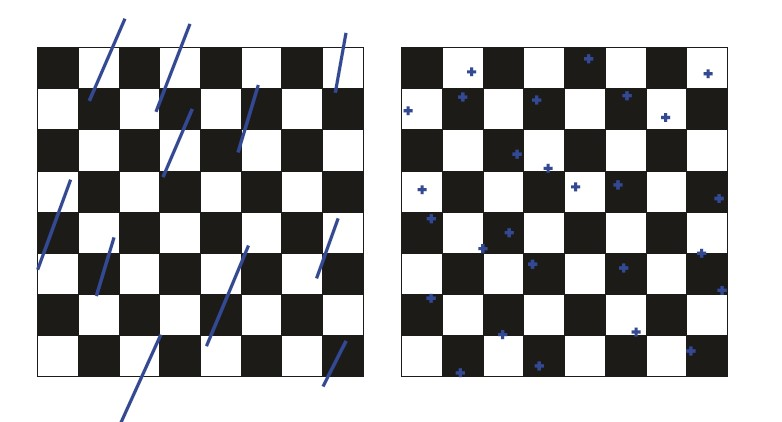
\includegraphics[width=0.5\textwidth]{Imagens/estatisticaDePoison.jpg}
		}%
		\caption{Estatísticas de Poisson. Esta classe de estatísticas pode ser descrita pela “analogia da gota de chuva” conforme mostrado acima. Isso é relevante para a radioterapia, pois a radiação que atinge as células é bastante semelhante a gotas de chuva atingindo uma placa.}
		\label{fig:estatisticaDePoison}
	\end{figure}

	$D_0$ é definido como a dose de radiação que resulta em 37\% de sobrevivência. Supõe-se que essa dose seja igual à dose de radiação necessária para causar um golpe letal por célula.
	
	O modelo de Poisson também é usado para probabilidade de controle de tumor (TCP):

	\begin{itemize}
		\item Em uma média de X células tumorais sobreviventes por paciente:
		\begin{itemize}[label=\textcolor{CarnationPink}{$\star$}]
			\item \textcolor{DarkTurquoise}{\textbf{$\mathbf{\left(e^{-X}\right)}$}}  pacientes são curados (nenhuma célula tumoral);
			\item \textcolor{DarkTurquoise}{\textbf{$\mathbf{\left(1 - e^{-X}\right)}$}} pacientes tiveram recorrência (no mínimo 1 célula tumoral)
		\end{itemize}

		\item Baseado nessa equação temos:
		\begin{itemize}[label=\textcolor{CarnationPink}{$\star$}]
			\item \textcolor{DarkTurquoise}{\textbf{1 célula tumoral por pcte:}} \textbf{TCP = 0.37}
			\item \textcolor{DarkTurquoise}{\textbf{0.5 célula tumoral por pcte:}} \textbf{TCP = 0.61}
			\item \textcolor{DarkTurquoise}{\textbf{0.1 célula tumoral por pcte:}} \textbf{TCP = 0.90}
			\item \textcolor{DarkTurquoise}{\textbf{0.05 célula tumoral por pcte:}} \textbf{TCP = 0.95}
			\item \textcolor{DarkTurquoise}{\textbf{0.01 célula tumoral por pcte:}} \textbf{TCP = 0.99}
		\end{itemize}
		\item \textcolor{DarkTurquoise}{\textbf{Regra prática:}} para atingir um determinado TCP, você deve apontar para uma sobrevivência de células tumorais de (1 - TCP).
	\end{itemize}


\section{Modelo de Alvo Único, Impacto Único}

	O modelo de sobrevivência celular "Single-Target, Single-Hit" (ou Modelo de Alvo Único, Impacto Único) é um modelo simplificado utilizado na radiobiologia para descrever a sobrevivência das células após a irradiação com radiação ionizante. Esse modelo assume que cada célula tem um único alvo crítico (como um núcleo celular) e que se atingido alvo leva à morte da célula.

	No modelo "Single-Target, Single-Hit", a resposta das células à radiação é binária: ou o alvo é atingido e a célula é inativada (morte celular) ou o alvo não é atingido e a célula permanece viva. Portanto, não leva em consideração a possibilidade de danos reparáveis no DNA ou outros efeitos colaterais da radiação.

	Para uma dada dose $\mathcal{D}$: 

	\begin{equation}
		SF(\mathcal{D}) = e^{-\mathcal{D}/D_0}
	\end{equation}

	\begin{exemplo}[onde:]
		\begin{itemize}
			\item \textcolor{DarkTurquoise}{\textbf{$D_0$}} (“D-Zero”) = dose necessária para causar 1 golpe letal por célula
			\item \textcolor{DarkTurquoise}{\textbf{$n$}} = 1.
			\item \textcolor{DarkTurquoise}{\textbf{$D_q$}} = 0.
			\item Quando você plota seus pontos de dados SF versus Dose em um gráfico semilog, seria uma linha reta, indicando que a sobrevivência é uma função exponencial da dose. Ou seja, uma linha reta em um gráfico semilog significa puramente morte exponencial que é definida apenas por $D_0$. 
			\item Se $\mathcal{D} = D_0$, $SF(\mathcal{D}) = e^{- D_0/D_0} = e^{-1} = 0.37$ que também é chamado \textcolor{DarkTurquoise}{\textbf{$D_{37}$}}
			\item Este tipo de curva de sobrevivência é visto para células de mamíferos que são irradiadas com radiação de alta LET (densamente ionizante), como partículas alfa ou íons de carbono; células muito sensíveis à radiação, como linfócitos e células da medula óssea; células que apresentam grandes defeitos no reparo da quebra da fita dupla do DNA; células que estão sincronizadas na fase M; e para células que têm reparo de quebra de fita dupla de DNA inibido quimicamente ou por supressão de genes.
		\end{itemize}
	\end{exemplo}

\section{Modelo de Múltiplos Alvos, Hit Único}

\section{Modelo Linear-Quadrático (LQ, Alfa-Beta)}

\section{Os “4 Rs” da Radiobiologia}

\section{Danos e Reparos}

\section{Taxa de Dose}



\bibliography{ref.bib}
\end{document}